\begin{frame}{Metodologia: Escopo}

\begin{itemize}
    \item<1->O escopo da pesquisa foi limitado ao estudo do \textbf{paradigma da primeira pessoa do singular no modo indicativo e no tempo presente}. Ex: (Eu) falo, gosto, ouço. \\
    \item<2->A tarefa proposta é a de prever uma forma verbal flexionada, dada uma forma primária (\textbf{Radical + Vocal Temática}). Por exemplo, para o verbo Amar:
    
    \begin{align*}
    \text{Am + a + r}\\
    \text{Radical + VT + Desinência de Infinitivo}\\\\ 
    \text{Am + a} \rightarrow \text{Amo} \\
    \text{Radical + VT} \rightarrow \text{Forma Flexionada}
\end{align*}
    
\end{itemize}

\end{frame}

\begin{frame}{Corpus}
\begin{itemize}
    \item<1->O \textit{corpus} produzido é composto por 423 verbos que foram marcados como pertencendo às famílias de verbos regulares (51\%) ou irregulares (49\%).
    \item<2->Dentro do escopo da família de verbos irregulares, foi possível identificar 15 subgrupos conforme a identificação de diferentes padrões de flexão.
\end{itemize}
\end{frame}

\begin{frame}{Modelo}

\begin{figure}
    \centering
    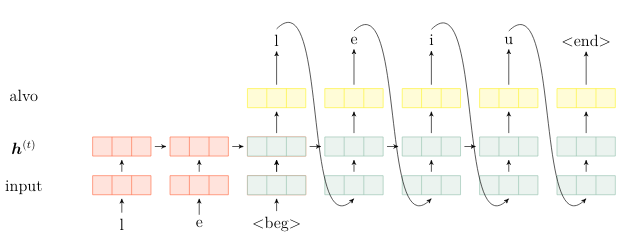
\includegraphics[width=0.8\textwidth]{images/metodologia/modelo.png}
    \caption{Esquema do Encoder-Decoder Desenvolvido}
    \label{fig:modelo}
\end{figure}

\end{frame}

\begin{frame}{Pré-Processamento}

\begin{figure}
    \centering
    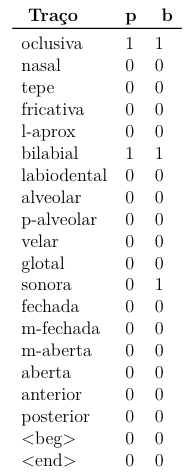
\includegraphics[width=0.2\textwidth]{images/metodologia/features.png}
    \caption{Exemplo de Codificação de fones}
    \label{fig:features}
\end{figure}
    
\end{frame}

\begin{frame}{Avaliação}

\begin{itemize}
    \item<1->A \textbf{Acurácia} foi a métrica escolhida para avaliar o modelo. Isso significa que o modelo deve prever corretamente todas as características fonéticas de cada fone do alvo.
    \item<2->Foram realizadas 30 análises K-fold com K=5.
\end{itemize}
    
\end{frame}